\section{Implementierung und Testszenarien}
Beschreibung des Kapitels

\subsection{Programmierung}
Die Implementierung erfolgte in C++. Zusätzlich wurden OpenCV als unterstützendes Framework genutzt. Die Grundlegende Klassenstruktur ist in Abbildung \ref{klassendiagramm} verdeutlicht.

\begin{figure}
\begin{centering}
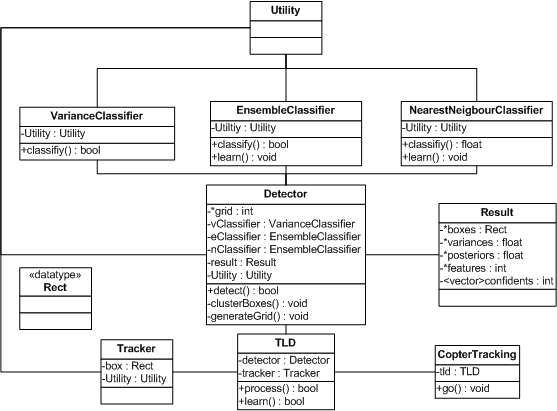
\includegraphics{../pictures/Klassendiagrammvsd.jpg}
\caption{Klassendiagramm zur Implementation mit den wichtigsten Attributen und Methoden}
\label{klassendiagramm}
\par\end{centering}
\end{figure}

\subsubsection{Klassenstruktur}
\paragraph{Klasse \textit{CopterTracking}}
Sie bildet den Einstieg ins Programm. Mittels OpenCV wird das Kamera- beziehnungsweise Videobild Frame für Frame eingelesen. Außerdem erfolgt hier die Definition des Objekts und die Übergabe des nächsten zu analysierenden Bildes sowie der Objektrepräsentation durch die aktuelle Box an die Klasse \textit{TLD}.

\paragraph{Klasse \textit{TLD}}
Diese Klasse bildet das Kernstück des Algorithmus und implementiert alle Methoden für das Zusammenspiel der Komponenten. Kernstück bildet die Funktion \textit{process()}, die als Eingabe aktuelle Bild $I$ mit der zuletzt gefundenen BoundingBox $b$ erwartet und die BoundingBox $b'$ berechnet, sofern das Objekt gefunden wird. Neben der Initialisierung aller Komponenten beim Start des Programms, implementiert sie auch die Auswertung der Ergebnismengen von Tracker und Detector in \textit{compareBoundingBoxes()}, die Beide unabhängig von einander die Daten verarbeiten. Das ist die Implementierung von P-N Learning (3.3).

\paragraph{Klasse \textit{Tracker}}
Die Implementierung des MedianFlow-Trackers ist in dieser Klasse realisiert.

\paragraph{Klasse \textit{Detector}}
Diese Klasse implementiert die Kaskade aus den drei Classifiern \textit{VarianceClassifier}, \textit{EnsembleClassifier} und \textit{NearestNeigbourClassifier}. Weiterhin hält der Detector das Model des gesuchten Kopters als \textit{Result}-Objekt vor und berechnet in der Funktion \textit{clusterBoxes()} die Cluster, aus denen dann ein oder mehrere finale Boxen berechnet werden. Initial definiert der Detector mittels der Funktion \textit{generateGrid()} das \textit{Grid} als eine \textbf{int}-Zeigervariable, die Grundlage des sliding-window-Ansatzes ist. Es hat sich während der Implementierung gezeigt, dass eine Indexierung auf einer Zeigervariable die Abarbeitungsgeschwindigkeit gegenüber einer Implementierung des Grids in Form eines Vector-Objekts stark erhöht.

\paragraph{Klasse \textit{VarianceClassifier}}
In einer Schleife werden nacheinander alle durch das \textit{Grid} gegebene Windows mittels Klassifizierer-Kaskade bewertet. Die erste Stufe, bildet dies Klasse VarianceClassifier. Die Methode \textit{classify()} zeichnet sich für die Bewertung verantwortlich und füllt die entsprechenden Varianz-Werte des \textit{Result}-Objekts.

\paragraph{Klasse \textit{EnsembleClassifier}}
Stufe zwei der Kaskade ist durch die Klasse \textit{EnsembleClassifier} definiert, die im Detail den vorgestellten \textit{FernClassifier} repräsentiert. Auch diese hat eine \textit{classify()}-Methode, vefügt jedoch zusätzlich über eine \textit{learn()}-Methode, über die der Klassifizierer in der Lernphase trainiert wird.

\paragraph{Klasse \textit{NearestNeigbourClassifier}}
Die letzte Stufe ist der \textit{NearestNeigbourClassifier} mit den zur Klassifizierung und zum Trainieren benötigten Methoden \textit{classify()} und \textit{learn()}. Neben der Nutzung im Detector dient er auch zur Bewertung der Tracker- und Detector-Box durch die \textit{P-N Learning}-Komponente in der \textit{TLD}-Klasse für die Lernphase.

\paragraph{Klasse \textit{Result}}
Während der Bewertung jeder einzelnen Box durch die Kaskade der drei Classifier, werden neben der eigentlichen Klassifizierung, auch die ermittelten Werte (variance, posteriors, confidence) und die durch ein Rechteck defininierte Box in einem Result-Objekt zwischengespeichert. Die berechneten Werte werden in Zeiger- beziehnugsweise Vector-Variablen gespeichert. Vor allem erstere bieten einen sehr schnellen Speicherzugriff und damit eine laufzeitstarke Abarbeitung von TLD.

\paragraph{Klasse \textit{Utility}}
Diese Klasse liefert eine Reihe Klassenmethoden für unterschiedliche Berechnungen, die an verschiedenen Stelle im Programm genutzt werden.

\paragraph{Zusätzliche Angaben}
In den ersten Versionen des Programms wurde ein streng objektorientierter Ansatz verfolgt. Das bedeutet, dass das Objekt-Modell auch als eine solche Klasse definiert war. Und alle Objekte bildeten wiederum eine Grid, das als Vector-Variable hinterlegt war. Wie sich allerdings gezeigt hat, war die Abarbeitungsgeschwindigkeit bei einem großen Grid und damit einer Menge von Objekten nicht zufriedenstellend. Trotz Übergabe des Grids als call-of-reference-Zeigervariable war nur mit einer kleinen Gridgröße von maximal 4000 Objekten eine passable Abarbeitung möglich. Dies entsprach allerdings bei weitem nicht der in der originalen Matlab-Implementierung beschriebenen ca. 50.000 Boxen. Indexierungen über Zeigervariablen sind um ein Vielfaches schneller und deshalb wurde ein Refactoring durchgeführt, in dem alle laufzeitkritischen Vector-Variablen durch Zeiger ersetzt wurden. Die Herausforderung bestand im Anschluss darin, eine möglichst geschickte Indezierung zu erzeugen, das zum Teil mehrdimensionale Werte in einer eindimensionalen Variable hinterlegt werden müssen.

\subsection{Lern- und Testphasen}
\label{subsection:learning_and_testing}
Die Ergebnisse der originalen Implementation von TLD mittels Matlab sind beeindruckend...(HIER NOCH ETWAS ZU DEN ERGEBNISSEN). Aus diesem Grund viel die Wahl auf TLD.

Nach der Implementation sollte die Eignung von TLD auf das Koptertracking getestet werden. Dazu wurden verschiedene Testszenarien erstellt und durchgespielt, die nun kurz vorgestellt werden.

Als Datenquelle dienten in erster Linie Video- und Kamerasequenzen, die mittels einer handelsüblichen SRL in einer Auflösung von $640\times480$ Pixel aufgenommen wurden. Als Modell wurde der \textit{MINI-QUADROCOPTER QG 550 XS} gewählt (BILD). Es sollten vor allem zwei wesentliche Dinge überprüft werden:

\begin{enumerate}
\item Unter welchen Umständen bezwiehungsweise welche Kriterien müssen erfüllt werden, damit ein Kopter erfolgreich gefunden und verfolgt werden kann.
\item Kann durch spezielle Lernphasen und damit einer Verfeinerung des Models der Erfolg des Trackens verbessert werden.
\end{enumerate}

\subsubsection{Videosequenzen}
Die verwendeten Videosequenzen decken Szenarien ab, in denen ein Kopter getrackt werden muss. Es wurden verschiedene mögliche negative Einflussfaktoren wie Änderungen der Lichtverhältnisse, wechselnde Bewegungsgeschwindigekeiten und Bewegungsrichtungen mit Innen- und Außenaufnahmen simuliert. Neben der manuellen Initialisierung von TLD durch den Nutzer, dienten die in den Szenen erzeugten Models in einigen Testläufen ebenfalls als Initialisierung und wurden zusätlich erweitert.

Da TLD bereits durch verschiedene, zum Download zur Verfügung stehende Evaluierungssequenzen getestet worden ist, und es für den speziellen Fall des Kopter-Trackings keine Daten vorhanden waren, wurden ausschließlich eigene Sequenzen verwendet.

\subsubsection{Kamerasequenzen}
Da Videosequenzen nur bedingt für die Verfeinerung eines Models geeignet sind, wurden zuätlich Kamerasequenzen genutzt. Dadurch kann auf Tracking-Detection-Probleme und der Verfälschung des Models durch fehlerhafte Fokussierung von TLD reagiert werden.